\documentclass[UTF8, xcolor=table]{beamer}
%\usepackage{fontspec}
%\setsansfont{宋体}
\usepackage[BoldFont,SlantFont]{xeCJK}
\setCJKmainfont[BoldFont={SimSun},ItalicFont={SimSun}]{SimSun}
\usepackage{latexsym,amssymb,amsmath,amsbsy,amsopn,amstext,xcolor,multicol}
\usepackage{graphicx,wrapfig,fancybox}
\usepackage{pgf,pgfarrows,pgfnodes,pgfautomata,pgfheaps,pgfshade}
\usepackage{thubeamer}
%\usepackage[backend=bibtex,style=IEEE,sorting=none]{biblatex} % [参考文献格式](https://www.sharelatex.com/blog/2013/07/31/getting-started-with-biblatex.html)
\usepackage[backend=bibtex,sorting=none]{biblatex} % [参考文献格式](https://www.sharelatex.com/blog/2013/07/31/getting-started-with-biblatex.html) %mac IEEE not found
\usepackage{array}
\usepackage{bm}
\usepackage{caption}
\usepackage[caption=false,font=scriptsize]{subfig}
\usepackage{multirow}
\usepackage{booktabs}
\usepackage{tikz}
\usepackage{tikzscale}
\usepackage{animate}
%\usepackage{times} %与上面的冲突,加上这个 粗体斜体就失效
%\usepackage{mathptmx}


\defbibheading{bibliography}[\bibname]{} %avoid printbibliography 自动生成目录
\addbibresource{ref/papers-bib-in-google.bib}
\addbibresource{ref/chinese-ref.bib}
%\setbeamertemplate{bibliography item}{\insertbiblabel} %将列表中默认的丑陋的icon 改成数字,或者下面这个也行
\setbeamertemplate{bibliography item}[text] % [ref](http://tex.stackexchange.com/questions/68080/beamer-bibliography-icon)
%\setbeamertemplate{footline}[frame number]{}

%\setframeofframes{of}

\usepackage{boxedminipage} %for: bvh border
\def\fourgraphicswidth{0.35} %0.3\textwidth

\usepackage{algorithm} %%format of the algorithm
\usepackage{algpseudocode}
\floatname{algorithm}{算法}
\renewcommand{\algorithmicrequire}{\textbf{输入:}} %%Use Input in the format of Algorithm
\renewcommand{\algorithmicensure}{\textbf{输出:}} %%UseOutput in the format of Algorithm
%\algrenewcommand{\algorithmiccomment}[1]{\hskip3em $\rightarrow$ #1}
\algrenewcommand{\algorithmiccomment}[1]{ $//$ #1}

\usepackage{listings}
\renewcommand\lstlistingname{代码}
\renewcommand\lstlistlistingname{代码}

\lstset{framexleftmargin=1.4em,
        xleftmargin=1.8em,
        basicstyle=\ttfamily\small,
        %frame=shadowbox, numberstyle=\tiny, breaklines=true,
        frame=single,
        numberstyle=\tiny, breaklines=true,
        keywordstyle=\color{blue!70}\bfseries,
        %commentstyle=\color{red!50!green!50!blue!50},
        rulesepcolor=\color{red!20!green!20!blue!20},
        numbers=none,fontadjust=true}
\lstdefinelanguage{shader}{morekeywords={uniform, layout, uniform, vec2, vec3, vec4, in, out, gl_Position, dot, flat, int ,float, gl_VertexID, xyz, w, x, y, z, location, version, sampler2DRect, bgr, gl_FragData, texture2DRect, gl_TexCoord,for,xy},morecomment=[l]{//}}

%\setbeameroption{show notes} %un-comment to see the notes

%\usepackage{pgfpages}
%\renewcommand\pgfsetupphysicalpagesizes{%
%    \pdfpagewidth\pgfphysicalwidth\pdfpageheight\pgfphysicalheight%
%}
%\setbeameroption{show notes on second screen}

\begin{document}

\setbeamerfont{footnote}{size=\tiny}
\setbeamerfont{caption}{size=\scriptsize}
\setbeamertemplate{caption}[numbered]
\setbeamerfont{subsection in toc}{size=\footnotesize}
\renewcommand*{\bibfont}{\footnotesize}

\graphicspath{{figures/}}

\title{Towards zero loss for TCP in wireless networks}
%\author{唐磊}
\author[董泽锋]{(申请西南交通大学工学硕士学位论文答辩报告)\vskip 20pt学~~~~~~生:董~~~~~泽~~~~~锋\vskip 5pt 指导教师:陈~~庆~~春~~教授}
\institute[西南交通大学~信息学院]{\small \vskip 38pt信息编码与传输重点实验室 }
%\date{2015-06-07}
\date{\small \vskip -17pt二〇一七年五月}
%\date{\today}



\frame{
\vspace{-15mm}
\titlepage
\vspace{-43mm}
\begin{figure}[htbp]
  \begin{center}
	
\includegraphics[width=0.14\linewidth]{swjtu.eps}
  \end{center}
\end{figure}
%\beign{picture}(1,1)
%\put(6,8){\includegraphics[width=0.15\linewidth]{Tsinghua_University_Logo.eps}}
%\end{picture}
}

  \section*{目录}
  \frame {
    \frametitle{\secname}
   % \begin{multicols}{2}
    \tableofcontents[sections={<1-5>}]
  %\end{multicols}
    \note{
      我将按照下面如下的次序来介绍本人的工作,首先是课题背景和相关工作,然后介绍凸包围体生成算法和基于凸包围体的碰撞检测算法,最后进行总结。
    }
  }

  \AtBeginSubsection[] {
  \frame<handout:0> {
  \frametitle{目录}
  \tableofcontents[current,currentsubsection,sections={<1-5>}]
    }
    \addtocounter{framenumber}{-1}  %目录页不计算页码
  }

  \section{背景}
  \frame
  {
    \frametitle{\secname~ }
    \begin{block}{TCP在无线网络中的局限性}
    	TCP最初是针对有线网络设计的,
    	其拥塞控制模型基于丢包设计。
    	由于无线网络误码率高,
    	传统TCP无法很好应对无线网络中的数据传输。
    \end{block}
    \begin{block}{TCP/NC}
    	Sundararajan等人提出TCP/NC\footfullcite{Sundararajan2009},
    	在OSI协议栈的TCP层和NC层添加一个网络编码层。
		在网络编码层对数据包进行冗余编码,
		掩盖链路中出现的丢包。
    \end{block}
    \note{
    }
  }

  \subsection{TCP/NC原理}
  \frame{
  \frametitle{TCP/NC框图}
      \begin{columns}[onlytextwidth]
      	%%\vspace{5em}
      	\hspace{-3.0em}
      	\begin{column}{0.55\textwidth}
      	  \begin{figure}
      		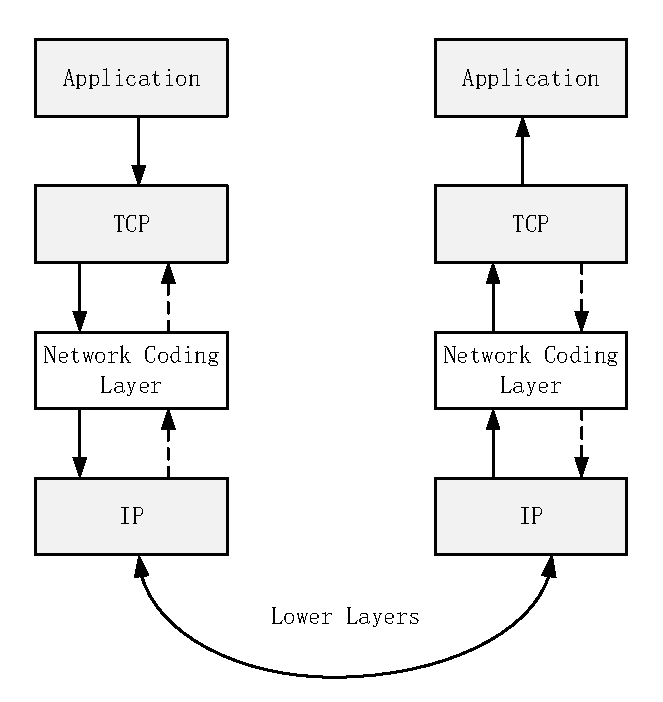
\includegraphics[height=5cm]{../figures/tcpnc.eps}
      		\caption{TCP/NC结构框图}
      		\label{fig:tcpnc}
      	\end{figure}
      	\end{column}
      \hspace{0.5em}
      \begin{column}{0.55\textwidth}
      	\footnotesize
      	\begin{block}{NC层发送端}
      		接收TCP层的数据包,
      		根据编码窗口和冗余因子对数据包进行线性组合,然后发往IP层。
      		接收端收到足够线性组合包后就可以将原始数据包解码出来。
      	\end{block}
      \begin{block}{NC层接收端}
      	接收IP层传上来的编码包,
      	满足可解条件后,
      	将原始数据宝解码出来,
      	往上传给TCP层。
      \end{block}
      \end{column}
      \end{columns}

%        \vspace{-1em}
%      其他:Tribox、Swept-sphere、 Sphere-shell、Zonotopes、圆柱形、圆锥、椭球形等等。
%      
      \note{
        上面这几个就是最常见的凸包围体。最常见的沿坐标轴方向的AABB包围盒,带方向的包围盒OBB,包围球,k面的凸包围体(k-DOP),和凸包,还有一些比较特定领域用的圆柱、圆锥形、椭球形等等。
        其中k-DOP是采用k/2对固定方向的半空间相交构成的凸包围体,是综合比较较好的包围体,因为可以通过k来调节包围体的简单性和紧致性来满足不同应用的需求。
      }
  }
\frame{
	\frametitle{Seen Packet}
	\vspace{-2em}
	\begin{myDef}[See a packet]\label{def:seepkt}
		如果一个节点根据现有的信息可以计算出如\textbf{\emph{$\left(p+q\right)$}}形式的线性组合,
		那么我们就说这个节点“\textbf{see packet \emph{$p$}}”。
		其中\textbf{$q$}本身就是只包含序号比$p$大的报文的线性组合。
		解码出某个报文也算作是“\textbf{see a packet}”,此时\textbf{$q=0$}。
	\end{myDef}
	\vspace{+1em}
	例如,接收端收到编码包$C\left[1\right]=p_1+p_2+p_3+p_4$,
	由定义\ref{def:seepkt}可知,
	接收端看到了报文$p_1$。
	如果再次接收到$C\left[2\right]=p_1+2p_2+3p_3+p_4$,
	由$C\left[2\right] - C\left[1\right] = p_2+p_3$,
	由定义\ref{def:seepkt}可知,接收端看到了报文$p_2$。
	接收端对于看到的每个报文,
	都会回复给发送端一个ACK。
	
}
   \frame{
   \frametitle{编解码示例}
     \footnotesize%%字体
     \begin{columns}[onlytextwidth]
     	\hspace{-2.0em}
     	\begin{column}{0.55\textwidth}
     		\begin{figure}
     			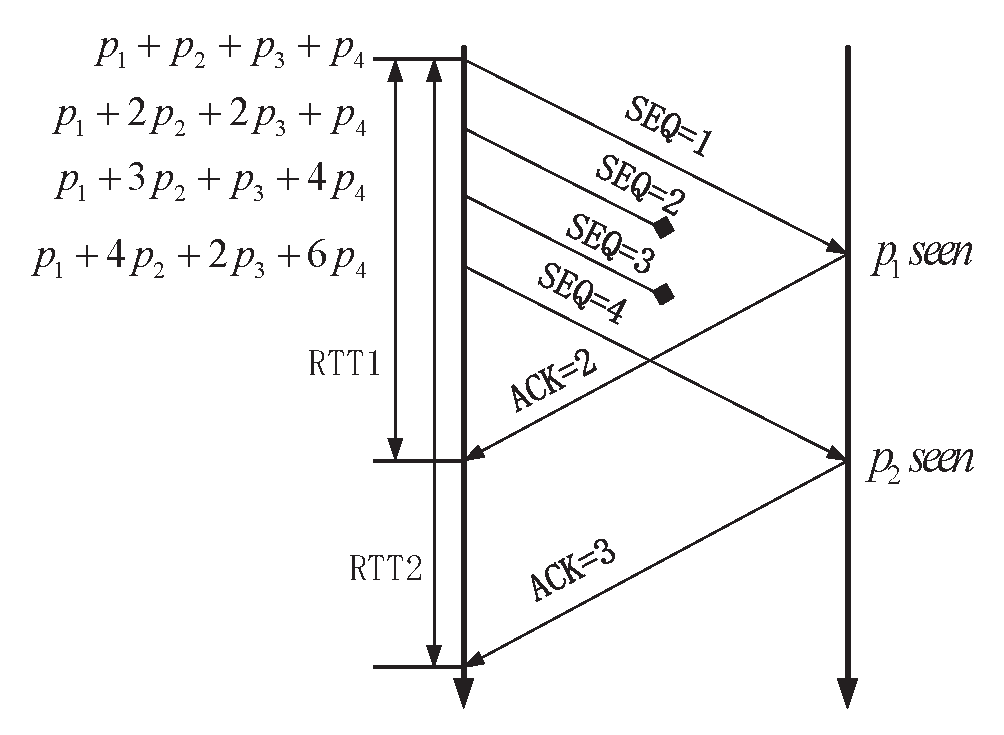
\includegraphics[height=5cm]{../figures/codingack.eps}
     			\caption{编码发送示例}
     			\label{fig:codingexp}
     		\end{figure}
     	\end{column}
     	\hspace{4.5em}

     	\begin{column}{0.40\textwidth}
     		%\footnotesize
     		% \vspace{+15em}
     		如图\ref{fig:codingexp}所示,
     		尽管$SEQ=2$和$SEQ=3$丢失,
     		但是接收端在收到$SEQ=4$的编码包后,
     		看到了报文$p_2$,
     		所以回复给发送端的是$ACK=3$。
     		对于处于接收端未解出的报文,
     		如$p_3$和$p_4$,就交给后续的冗余包来补偿。
     		
     	\end{column}
     \end{columns}
%     \textbf{$k$-DOP}\footfullcite{klosowski1998efficient}的局限性:方向\textbf{固定}且为\textbf{有限的偶数},不同模型其截面方向一致, \textbf{不够紧致};\\ 
%     而凸包很(最)紧致,但面片数量太多,构造复杂度$O(n\log n)$。
%    \begin{block}{本文凸包围体的目标}
%      \hspace{-2.0em}   \begin{minipage}{\textwidth}
%    \begin{description}
%      \item[紧致:] 能够自适应模型,根据模型形状特点有不同的方向;
%      \item[快速:] 生成凸包围体的速度要快,利用~GPU~加速;
%      \item[灵活:] 通过参数~$k$~调节凸包围体的简单性和紧致程度。
%    \end{description}
%  \end{minipage}
%    \end{block}

       \note{
       }
  }

  \subsection{TCP/NC存在问题}
   \frame{
   \frametitle{传输时延 }
    \vspace{-1em}
    \begin{myDef}[传输时延]\label{def:shiyan}
    	如果源节点产生数据报文$pkt_i$的时间为$t_{s_i}$,
    	目的节点将数据报文$pkt_i$交付给上层时间为$t_{r_i}$,
    	定义数据包的传输时延为$delay_i=t_{r_i} - t_{s_i}$。
    \end{myDef}
   \begin{block}{解码导致的时延}
   	TCP/NC的基本思想是利用发送端的编码将链路的丢包问题后延,
   	当发送端的冗余包足够弥补链路丢包后,
   	丢包就被掩盖。
   	带来的问题是数据包的传输时延变大。
   	以图\ref{fig:codingexp}为例,
   	如果补偿$SEQ=2$的冗余包为$SEQ=7$,
   	那么$p_2$需要等到$SEQ=7$才能被接收端的NC层交付给上层TCP。
   	那么$p_2$的传输时延为$delay_2 = t_{r_7} - t_{s_2}$。
   	   \end{block}

%   \begin{block}{分类}
%     \begin{description}
%       \item[加速结构:] SPT(如四叉树、KD~树等)~v.s~\textbf{BVH}(OBB树、$k$-DOP树等)
%       \item[表现形式:] \textbf{刚体}~v.s~可变形,凸体~v.s~凹体,CSG~v.s~参数曲面~v.s~\textbf{多边形网格}
%       \item[碰撞环境:] \textbf{成对}~v.s~\textbf{多体},\textbf{静止}~v.s~\textbf{运动},\textbf{离散}~v.s~连续
%     \end{description}
%   \end{block}
   
   \note{
    (介绍PPT后),本文后面的实验就是基于BVH的,不可变形的三角网格。//现在研究较多的是连续的可变形的碰撞检测布料模拟头发模拟等。
   }
  }
%
%  \frame{
%    \frametitle{基于~BVH~的碰撞检测算法}
%    \begin{columns}[onlytextwidth]
%      \begin{column}{0.35\textwidth}
%        \vspace{-1.5em}
%        \begin{figure}[htbp]
%            \begin{center}
%            \begin{boxedminipage}{1\textwidth}
%            \subfloat{\label{lbl:bvh-bunny-center-0.png}}
%              {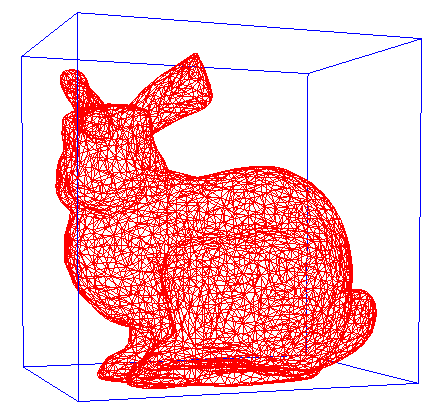
\includegraphics[height=1.4cm]{bvh-bunny-center-0.png}}
%            \subfloat{\label{lbl:bvh-bunny-center-1.png}}
%              {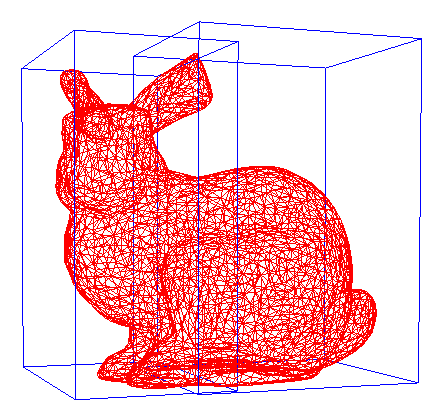
\includegraphics[height=1.4cm]{bvh-bunny-center-1.png}}
%            \\
%            \subfloat{\label{lbl:bvh-bunny-center-2.png}}
%              {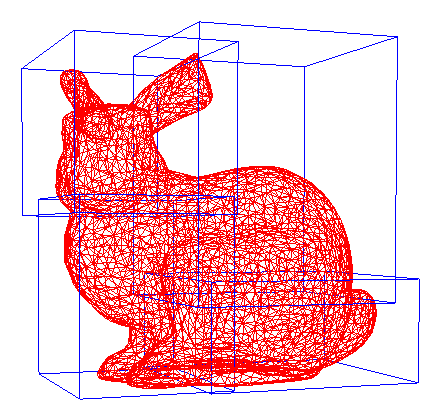
\includegraphics[height=1.4cm]{bvh-bunny-center-2.png}}
%            \subfloat{\label{lbl:bvh-bunny-center-3.png}}
%              {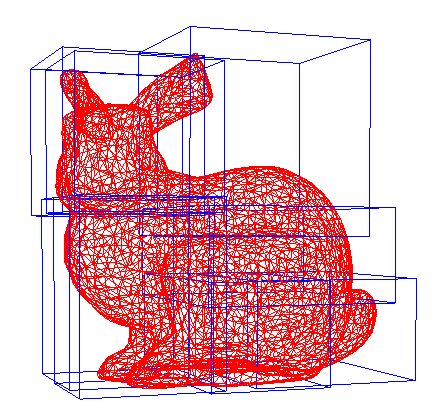
\includegraphics[height=1.4cm]{bvh-bunny-center-3.png}}
%            \\\hspace{0.5cm}
%            \subfloat{\label{lbl:bvh-bunny-center-4.png}}
%              {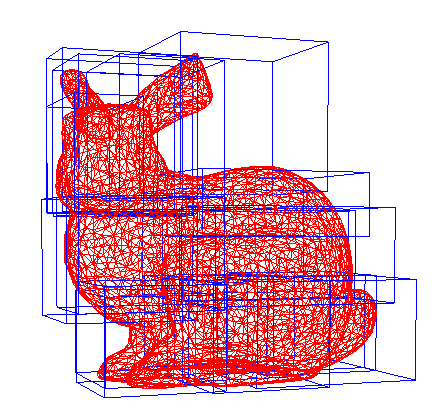
\includegraphics[height=1.5cm]{bvh-bunny-center-4.png}}
%            \subfloat{\label{lbl:bvh-bunny-center-5.png}}
%              {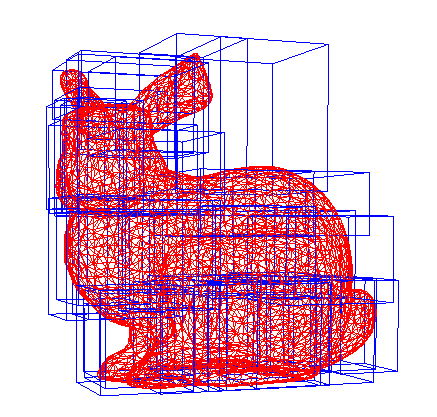
\includegraphics[height=1.5cm]{bvh-bunny-center-5.png}}
%            \\
%            \subfloat{\label{lbl:bvh-bunny-center-6.png}}
%              {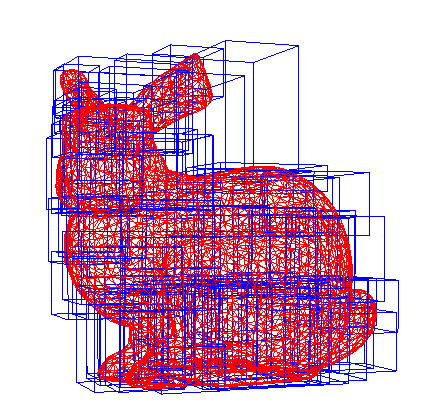
\includegraphics[height=1.5cm]{bvh-bunny-center-6.png}}
%            \subfloat{\label{lbl:bvh-bunny-center-7.png}}
%              {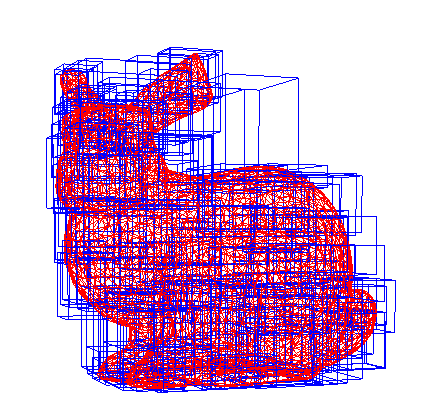
\includegraphics[height=1.5cm]{bvh-bunny-center-7.png}}
%            \end{boxedminipage}
%            \vspace{-0.5em}
%          \caption{八层~BVH~示例}
%          \label{lbl:bvh-example}
%          \end{center}
%          \end{figure}
%      \end{column}
%      \hspace{0.5em}
%      \begin{column}{1.2\textwidth}
%      \vspace{0.2em}
%         \scalebox{0.5}{
%              \begin{minipage}{1.0\textwidth}
%      \vspace{-2em}
%           \begin{algorithm}[H]
%              \caption{自顶向下层次遍历~BVH~}
%              \label{alg:traverse-bvh-tree}
%              \begin{algorithmic}[1]
%              \Require
%              两个~BVH~树的根节点~$node_1$,$node_2$
%              \Ensure
%              模型是否相交
%              \Function {TraverseBVHTree}{$node_1, node_2$}
%                \If{$node_1.bv \cap node_2.bv = \emptyset$}
%                  \State \Return{\textbf{False}}
%                  \Comment{包围体重合测试, 包围体不相交直接返回}
%                \Else
%                    \If {$node_1.children = \emptyset$}
%                         \If {$node_2.children = \emptyset$}
%                         \State \Comment{最底层叶子节点原生几何相交测试}
%                         \State \Return {\Call{CheckIntersection}{$node_1.primitives, node_2.primitives$}}
%                         \Else
%                            \ForAll {$child \in node_2.children$}
%                            \State \Call{TraverseBVHTree}{$node_1, child$} \Comment{递归调用}
%                            \EndFor
%                         \EndIf
%                    \Else
%                         \ForAll {$child \in node_1.children$}
%                         \State \Call{TraverseBVHTree}{$child, node_2$}  \Comment{递归调用}
%                         \EndFor
%                    \EndIf
%                \EndIf
%              \EndFunction
%              \end{algorithmic}
%              \end{algorithm}
%              \end{minipage}
%            }
%      \\
%      \scriptsize \hspace{1em}代价函数: $T_{cost} = n_v * C_v + n_p * C_p + (n_u * C_u)$(运动)
%      \end{column}
%    \end{columns}
%    \note{
%      基于包围体树的碰撞检测算法, 一般首先都会初始化环境然后构建层次结构的包围体树,碰撞检测时从顶层开始逐渐往下层遍历,到最底层叶子节点后开始三角网格模型相交测试,
%      当发现三角网格相交后立即终止遍历,确定模型发生碰撞。
%      评价碰撞检测算法的指标一般用上面这个公式来衡量,其中nv和 np分别表示参与包围体节点相交测试的数量和参与原始几何相交测试的数量,Cv和 Cp则表示相应的平均测试耗费的代价。
%      当在运动场景时还需要加上nu和 Cn就是模型旋转或者运动后包围体更新的数量和更新的代价。
%      本文算法就是尽早发现包围体不相交的情况,减少np和cp的数量。
%    }
%}

  
%    \section{总结与展望}
%    %添加一个目录
%    \frame{
%     \frametitle{目录}
%     \tableofcontents[current,currentsection,sections={<1-5>}]
%     \addtocounter{framenumber}{-1}  %目录页不计算页码
%    }
%
%    \frame{
%      \frametitle{\secname}
%      \vspace{-0.5em}
%      \begin{block}{总结}
%        \footnotesize
%        \begin{enumerate}[(1)]
%          \item 提出了一种构造紧致凸包围多面体--$k$-CBP~的算法;
%          \item 构造~$k$-CBP~速度上比现有算法快~3$\sim$8~倍;
%          \item 构造的~$k$-CBP~紧致程度比现有的$k$-DOP紧致10\% $\sim$ 40\%;
%          \item 提出了一种基于~$k$-CBP~的碰撞检测算法,该算法较$k$-DOP树算法初始化时间快8倍以上,静止场景快0.8 $\sim$ 3.2 倍,运动场景快0.8 $\sim$ 5.6 倍。
%        \end{enumerate}
%      \end{block}
%      \vspace{-0.5em}
%      \begin{block}{展望}
%        \footnotesize
%      \begin{enumerate}[(1)]
%          \item 碰撞检测算法如何摆脱对AABB树的依赖;应用于近似碰撞检测算法;应用于可变形的模型连续碰撞检测,如何快速更新~$k$-CBP~;
%          \item 如何将~$k$-CBP~应用于如机器人抓取、路径规划等其他应用领域中。
%        \end{enumerate}
%      \end{block}
%      
%      \note{
%        总结一下~\ldots PPT
%      }
%    }

%    \section{主要参考文献}
%    \frame[t,allowframebreaks]{
%      \frametitle{\secname}
%    \printbibliography
%    }
    
    \section{Q\&A}
%    \frame{
%      \frametitle{\secname}
%      \begin{block}{致谢}
%        \begin{enumerate}[(1)]
%          \item 导师雍俊海老师的精心指导;
%          \item 施侃乐老师帮助;
%          \item 研究所各个项目的历练;
%          \item 王斌老师、陈莉老师的评审及意见,答辩委员会老师聆听和指导。
%        \end{enumerate}
%      \end{block}
%    }
    \frame{
      \frametitle{Q \& A}
      \begin{block}{Questions?}
       ~\\ ~\\
       \center{\Large{Thank you!}}
       \\ ~\\ ~\\ ~\\ ~\\ 
      \end{block}
    }



\end{document}

